\documentclass[10pt]{cls/LaTeX-Class-File-for-Research-Report-Formats-of-Mahidol-University}
\usepackage[utf8]{inputenc}
\graphicspath{ {images/} }
\begin{document}
\typeOfReport{thematic} %thesis %thematic
\title{an implementation of latex class file for research report formats of mahidol university}
\titleThai{\begin{thai} การพัฒนาคลาสของ Latex เพื่อใช้ในการจัดรูปแบบรูปเล่ม วิทยานิพนธ์ หรือ สารนิพนธ์ ของมหาวิทยาลัยมหิดล  \end{thai}}
\author{Test Name-Lastname}
\authorThai{\begin{thai} ทดสอบ ชื่อ-นามสกุล \end{thai}}
\degreefaculty{M.Sc. (Information Technology Management)}
\degreefacultyThai{\begin{thai} วท.ม. (การจัดการเทคโนโลยีสารสนเทศ) \end{thai}}
\ProgramTitle{a thematic paper submitted in partial fulfillment of the requirements for the degree of master of science (information technology management) faculty of graduate study mahidol university 2017}
\DegreeTitle{Thematic Paper}
\SubmittedFor{Master of Science (Information Technology Management)}
\SubmittedDate{January 1, 2017}
\Advisor{Lect. Somchai Saijai, Ph.D. (Electrical Engineering)}
\CoAdvisor{Asst. Prof. Sakarin Daoray, Ph.D. (Electrical and Computer Engineering)}
\Committee{Asst. Prof. Sakarin Daoray, Ph.D. (Electrical and Computer Engineering)}
\CommitteePosition{Program Director Master of Science Program in Information Technology Management Faculty of Engineering Mahidol University}
\dean{Prof. Precha Prache, M.D.,Ph.D. (Biochemistry)}
\deanPo{Faculty of Graduate Studies, Mahidol University}
\deanAct{Asst. Prof. Warakorn Charoensuk, Ph.D. (Electical Engineering)}
\deanActPo{Faculty of Graduate Studies, Mahidol University}
\memberOne{Lect. Somboon Boonnad Ph.D. (Information Technology)}
\memberTwo{Asst. Prof. Kaijoh Brother, Ph.D. (Electrial and Computer Engineering)}
\memberThree{Asst. Prof. Sakarin Daoray, Ph.D. (Electrical and Computer Engineering)}

\referencesOrBibliography{References} %change name of title References Or Bibliography

\maketitle

\abstractCommittee{THEMATIC PAPER ADVISORY COMMITTEE: Prof}
\abstractEng{ABSTRACT ENG ABSTRACT ENG ABSTRACT ENG ABSTRACT ENG ABSTRACT ENG ABSTRACT ENG ABSTRACT ENG ABSTRACT ENG ABSTRACT ENG ABSTRACT ENG ABSTRACT ENG ABSTRACT ENG ABSTRACT ENG ABSTRACT ENG ABSTRACT ENG ABSTRACT ENG ABSTRACT ENG ABSTRACT ENG ABSTRACT ENG ABSTRACT ENG ABSTRACT ENG ABSTRACT ENG ABSTRACT ENG
}
\keywordEng{KEY WORDS: TEST}
\pageCountEng{32 pages}

\abstractCommitteeThai{\begin{thai} คณะกรรมการที่ปรึกษาสารนิพนธ์ : อาจารย์ \end{thai}}
\abstractThai{\begin{thai}
ส่วนภาษาไทย ส่วนภาษาไทย ส่วนภาษาไทย ส่วนภาษาไทย ส่วนภาษาไทย ส่วนภาษาไทย ส่วนภาษาไทย ส่วนภาษาไทย ส่วนภาษาไทย ส่วนภาษาไทย ส่วนภาษาไทย ส่วนภาษาไทย 
\end{thai}}
\keywordThai{}
\pageCountThai{\begin{thai}32 หน้า \end{thai}}
\begin{acknowledgement}
Your acknowledgement

Your acknowledgement

Your acknowledgement
\end{acknowledgement}

%%%%% please use it for header numbering mahidol style %%%%%
\maketitle
\tableofcontents
\listoftables
\listoffigures
\pagestyle{mahidol-fancy-style}

\chapter{Demo}
This is Demo of LaTeX-Class-File-for-Research-Report-Formats-of-Mahidol-University. You can read and do follow below.
\section{section}
\subsection{subcection}
\subsubsection{subsubsection}

\subsection{Demo itemize}
\begin{itemize}[topsep=0pt,itemsep=-1ex,partopsep=1ex,parsep=1ex,leftmargin=0pt,
itemindent=2.4cm]
\item[--] \textbf{bullet}
\item Normal font test bullet
\item \textbf{bold font test bullet}
\end{itemize}

\begin{thai}
 ทดสอบภาษาไทย \\
\end{thai}

\section{section}
\subsection{subcection}
Demo References \cite{latexproject}


\chapter{Demo Figure}
\section{Demo Figure}
Demo Figure \latex Software Structure shown in Fig. \ref{fig:fig1}

\begin{figure}[h]
  \centering
  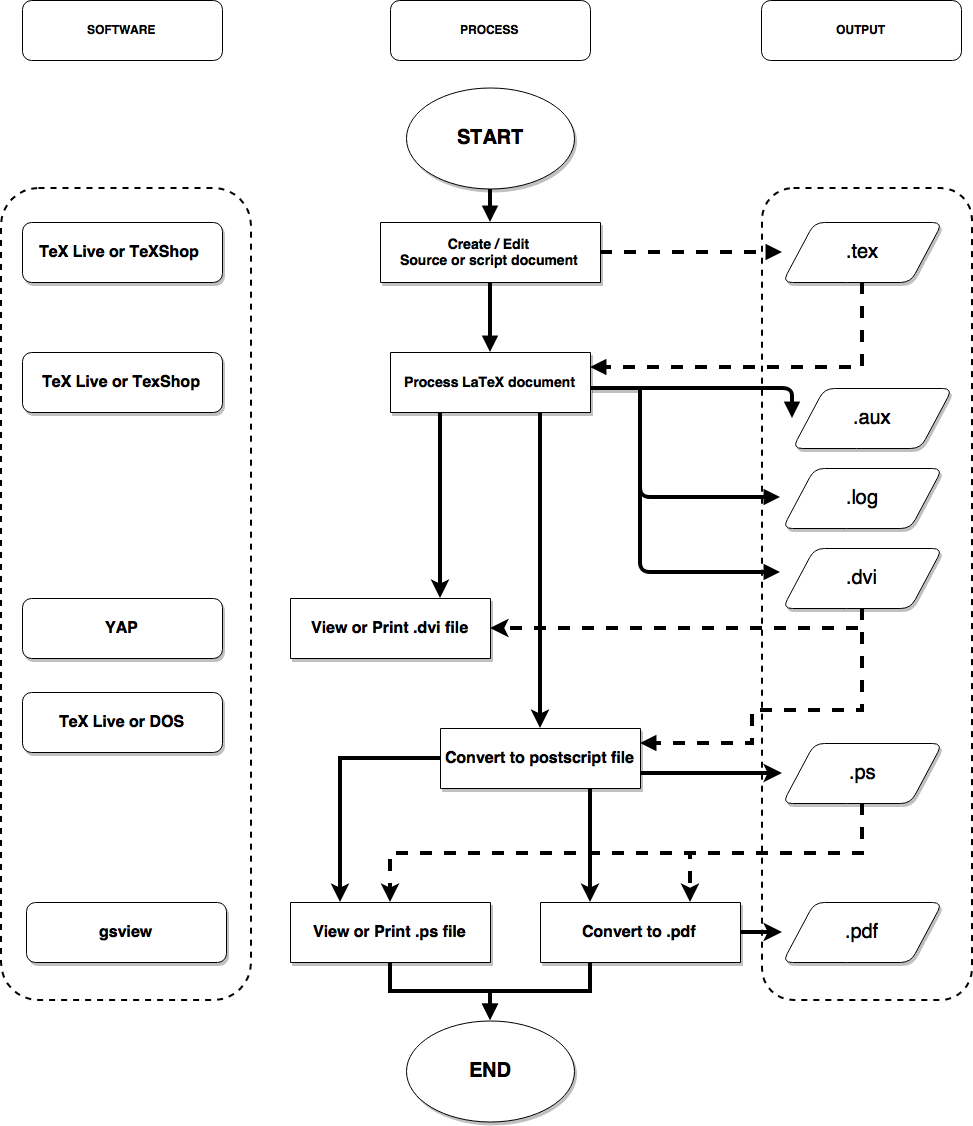
\includegraphics[width=12.00cm\linewidth]{LaTeX-Diagram-black-white.png}
  \caption{Demo Figure \latex Software Structure..}
  \label{fig:fig1}
\end{figure}

\section{Demo Figure}
Demo Figure 2 \latex Software Structure shown in Fig. \ref{fig:fig2}

\begin{figure}[h]
  \centering
  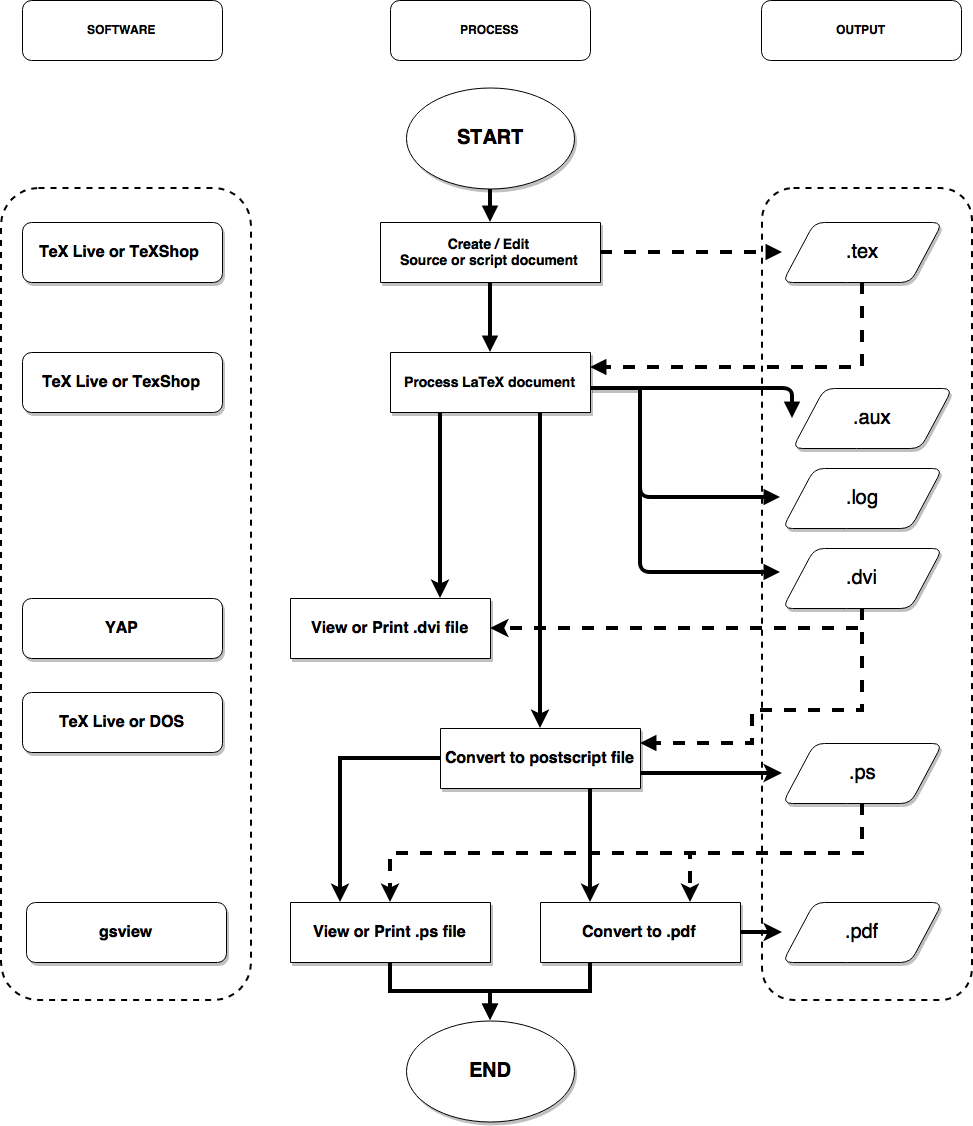
\includegraphics[width=12.00cm\linewidth]{LaTeX-Diagram-black-white.png}
  \caption{Demo Figure \latex Software Structure..}
  \label{fig:fig2}
\end{figure}
\chapter{Demo Table}
You can look at https://www.sharelatex.com/learn/Tables for learn or look at below

\section{Demo Table}
\begin{table}[ht]
\caption{Demo Table 1}
\begin{center}
\begin{tabular}{ |c|c|c| } 
 \hline
 cell1 & cell2 & cell3 \\ 
 cell4 & cell5 & cell6 \\ 
 cell7 & cell8 & cell9 \\ 
 \hline
\end{tabular}
\label{table:ta}
\end{center}
\label{table:ta}
\end{table}

\section{Demo Table 2}
\begin{table}[ht]
\caption{Demo Table 2}
\arrayrulecolor[HTML]{DB5800}
\centering
\begin{tabular}{ |s|p{2cm}|p{2cm}|  }
 \hline
 \rowcolor{lightgray} \multicolumn{3}{|c|}{Demo Table} \\
 \hline
 Demo Table \\
 \hline
 Afghanistan & AF &AFG \\
 \rowcolor{gray}
 Bangkok & bk	& bkk \\
 Loei	&lo	& le \\
 Ranong	&ra	& ron \\
 Trad & tr & trd \\
  \hline
\end{tabular}
\label{table:ta}
\end{table}
%\chapter{4}
%\chapter{5}
\begin{references}
    \vspace*{-2cm}
    \bibliographystyle{unsrt}
    \bibliography{references}
\end{references}
\begin{appendices}
\chapter{Appendix Test}

\section{Letter}
Letter font for use only black color crisp easy to read and use the same font throughout.

\chapter{Appendix Test2}

\section{Letter2}
Letter font for use only black color crisp easy to read and use the same font throughout.

\end{appendices}
\dateOfBirth{1 January 1900}
\placeOfBirth{Bangkok Thailand}
\institutionsAttended{Mahidol University}
\institutionsAttendedTwo{Mahidol University, 2015-2017 Master of Science (Information Technology Management)}
\homeAddress{99/999 Bangrak, Thailand 10540}
\tel{081-999-9999}
\email{test@test.com}
\office{Your company}
\employmentAddress{Place of work}

\biography

\end{document} %%%%%%%%%%  do not put anything after this
